% !TEX root = ../Dokumentation.tex
\subsection{Antrieb}

\textbf{Funktionsbeschrieb}\\[0.2cm]
Mit dem Antrieb ist der Hauptmotor gemeint, der an der Hinterachse montiert wird und für die Vor- sowie Rückwärtbewegungen des Fahrzeugs zuständig ist.
Die aktuelle Drehzahl des Motors wird von einem Encoder erfasst. Dieser wiederum sendet die gemessenen Daten an den Microcontroller der schlussendlich die Anzahl Umdrehungen reguliert.
.\\[0.2cm]
\textbf{Komponentenbeschrieb}\\[0.2cm]
\begin{figure}[h]
\centering
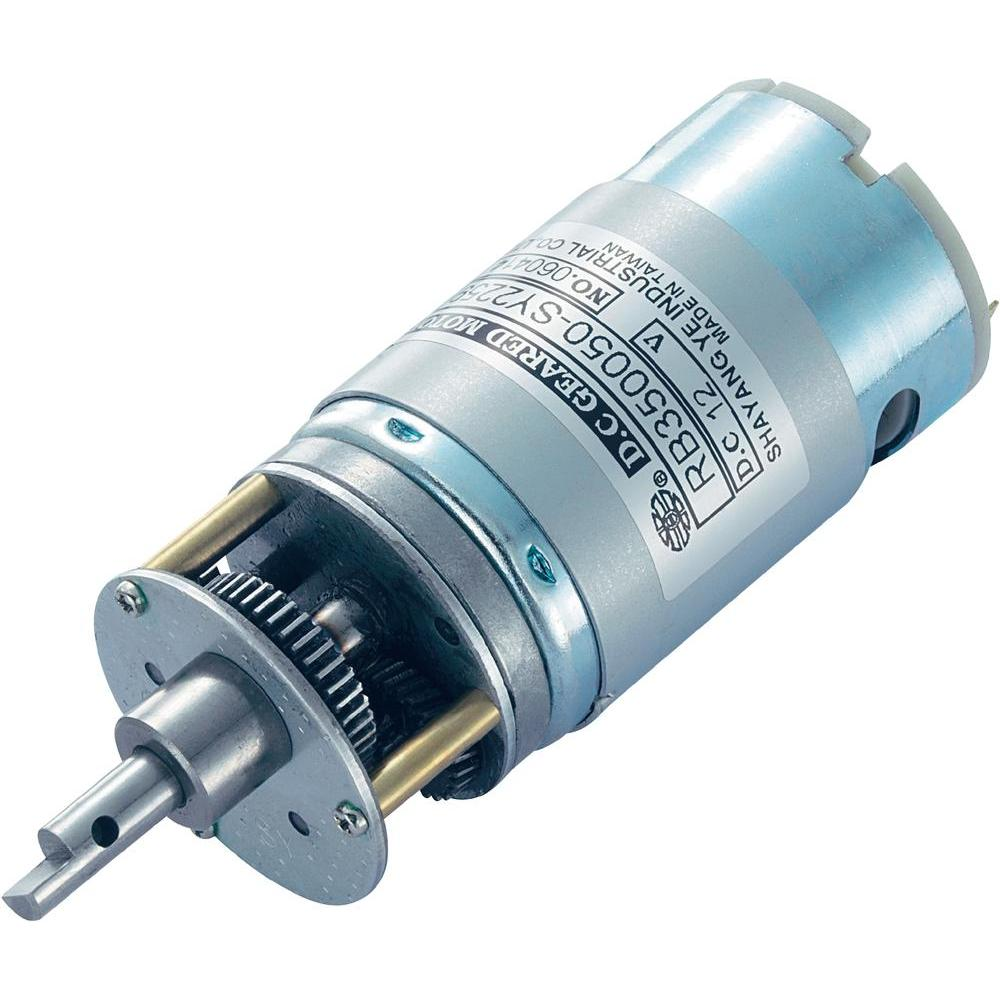
\includegraphics[width=0.5\textwidth]{03_Loesungskonzept/pictures/antrieb.jpg}
\caption{Antrieb  (Quelle:http://www.conrad.ch)}	
\end{figure}\\[0.2cm]
Als voraussichtlicher Favorit, wurde ein Hochleistungsgetriebemotor von Modelcraft ausgewählt. Die technischen Daten sind folgende:
\begin{itemize}
\item Leerlaufstrom: 0.32 A
\item Untersetzung: 18:1
\item Wellendurchmesser: 6 mm
\item Last-Drehzahl: 317 U/min
\item Leerlauf-Drehzahl an Nennspannung: 333 U/min
\item Betriebsspannung: 12 V DC
\item Spitzendrehmoment: 2.23 Nm
\item Max. Laststrom: 0.7 A
\item Durchmesser: 36 mm
\item Länge: 101.6 mm
\end{itemize}\\[0.2cm]
\textbf{Begründung}\\[0.2cm]
Der ausgewählte Motor punktet vor allem aufgrund seiner kleinen und kompakten Bauform. Dies ist einer der Hauptgründe für die Auswahl, da der Montageort für den Antrieb am Fahrzeug nicht verändert werden kann, ohne umständliche Wellen zu installieren und somit die Baugrösse einschränkt.
Ein weiter Punkt ist, dass er sich als Gleichstrommotor leicht ansteuern lässt und damit die Handhabung vereinfacht.
Zudem zeichnet er sich mit einer hohen Drehzahl und grossem Drehmoment aus und ist dennoch relativ günstig in der Anschaffung.\\[0.2cm]
\textbf{Berechnungen}\\[0.2cm]
Leistungsberechung:
\begin{itemize}
\item P = 2*\pi*N*M -> 2*\pi*5.258U/sec*2.23Nm = 73.98W


\end{itemize}